\documentclass[letterpaper,11pt,twoside]{article}
\usepackage[utf8]{inputenc}
\usepackage{amsmath,amsfonts,amssymb,amsthm,latexsym}
\usepackage[spanish,es-noshorthands]{babel}
\usepackage[T1]{fontenc}
\usepackage{lmodern}
\usepackage{graphicx,hyperref}
\usepackage{tikz,pgf}
\usepackage{multicol}
\usepackage{fancyhdr}
\usepackage[height=9.6in,width=7.1in]{geometry}
\usepackage{fancyhdr}
\pagestyle{fancy}
\fancyhead[LE]{
\includegraphics[height=12pt]{Images/logo-colegio.png} Aritmética $6^{\circ}$}
\fancyhead[RE]{}
\fancyhead[RO]{\textit{Germ\'an Avenda\~no Ram\'irez, Lic. U.D., M.Sc. U.N.}}
\fancyhead[LO]{}

\author{Germ\'an Avenda\~no Ram\'irez, Lic. U.D., M.Sc. U.N.}
\title{\begin{minipage}{.2\textwidth}

\includegraphics[height=1.75cm]{Images/logo-colegio.png}\end{minipage}
\begin{minipage}{.55\textwidth}
\begin{center}
Taller 09, Divisi\'{o}n en $\mathbb{N}$\\
Aritm\'{e}tica $6^{\circ}$
\end{center}
\end{minipage}\hfill
\begin{minipage}{.2\textwidth}

\includegraphics[height=1.75cm]{Images/logo-sed.png} 
\end{minipage}}
\date{}
\thispagestyle{plain}
\begin{document}
\maketitle
Nombre: \hrulefill Curso: \underline{\hspace*{44pt}} Fecha: \underline{\hspace*{2.5cm}}
 \section*{Aplico lo aprendido}
 \begin{minipage}{.3\textwidth}
  \begin{itemize}
 \item En la tienda de doña Rosario se encuentran los
siguientes productos.\\

Mario debe llevar: cinco kilos de arroz, tres docenas de
huevos, siete libras de tomate, cuatro libras de café, dos
paquetes de pasta, tres frascos de aceite, cuatro paquetes
de harina y ocho kilos de papa.
\end{itemize}
 \end{minipage}\hfill
 \begin{minipage}{.7\textwidth}
\begin{center}
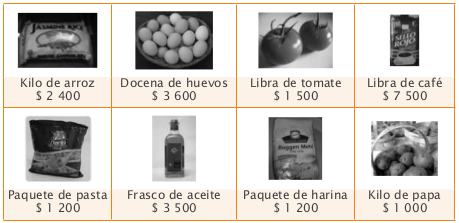
\includegraphics[scale=.76]{Images/productos.png} 
\end{center} 
 \end{minipage}
\begin{multicols}{2}
¿Mario podrá pagar sus compras con \$ 70\,000? ¿Por qué?
Mario decide pagar el valor total de sus compras en cuotas.
Si cada una es de \$ 17\,800, ¿cuántas cuotas debe pagar?
\begin{itemize}
\item Maritza compró ocho paquetes de almojábanas, pero
cuando empieza a desempacarlas se da cuenta que en vez
de tener las 72 unidades que esperaba sólo tiene 64.

¿Cuántas almojábanas pensaba Maritza que debía recibir
por paquete? ¿Cuántas almojábanas por paquete recibió
realmente Maritza?
\item Cinco toros con masas iguales pesan entre todos 2\,840
kg. ¿Cuál es el peso de cada uno?
\item A las fiestas patronales de Los Pinos asistieron 1\,253 hombres, 1\,786 mujeres y 175 menores de edad. Si la
plaza de toros del pueblo cobra \$ 15\,700 por la entrada
y se espera que asistan todos los visitantes, ¿cuánto se
recaudaría por entradas a la corrida de toros?
\item Para empacar 1\,500 huevos se dispone de bandejas en
cada una de las cuales caben doce unidades. ¿Cuántas
bandejas se necesitan?
\item Pilar hizo una llamada telefónica de doce minutos de
duración. Si le cobraron \$ 1\,500, ¿cuál es el costo de
cada minuto?
 \end{itemize}
\end{multicols}
\begin{minipage}{.35\textwidth}
 Observa la factura. Luego contesta las preguntas.
 \begin{itemize}
 \item ¿Cuál es el valor total de la factura?
\item ¿Cuál es el valor unitario de cada uno de los implementos comprados?
\end{itemize}
\end{minipage}\hfill
\begin{minipage}{.65\textwidth}
\begin{center}
\begin{tabular}{|c|c|c|c|}
\hline 
\textbf{Cantidad} & \textbf{Descripción} & \textbf{Valor unitario} & \textbf{Valor Total} \\ 
\hline 
5 & Cajas de puntillas & \$3\,500 & \$17\,500 \\ 
\hline 
3 & Cajas de tornillos & \$4\,200 & \$12\,600 \\ 
\hline 
50 & Chazos & \$100 & \$5\,000 \\ 
\hline 
20 & Tuercas & \$300 & \$6\,000 \\ 
\hline 
10 & Brocas & \$1\,500 & \$15\,000 \\ 
\hline 
\end{tabular} 
\end{center}
\end{minipage}
\begin{multicols}{2}
\begin{itemize}
\item ¿Cuál sería el costo de comprar tres cajas de puntillas, dos cajas de tornillos y
diez tuercas?
\item Si en un nuevo pedido se duplican las cantidades de implementos, ¿cuál es el valor de la nueva factura?
\end{itemize}
\end{multicols}
\begin{minipage}{.65\textwidth}
En un terreno de forma rectangular que tiene 15 m de ancho y 24 m de largo, cada metro cuadrado tiene un costo de \$ 250\,000.
\begin{itemize}
\item  Si se quiere cercar el terreno con tres hiladas de alambre de púas, ¿cuántos metros de alambre es necesario comprar?
\item  ¿Cuál es el precio total del terreno?
\item  Si se logra vender en \$ 98'550\,000, ¿cuál es la ganancia con respecto al precio inicial?	
\end{itemize}
\end{minipage}\hfill
\begin{minipage}{.35\textwidth}
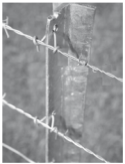
\includegraphics[scale=1]{Images/terreno_a.png} 
\end{minipage}
En la cosecha del mes de marzo, en una finca se recogieron las siguientes cantidades; 756\,205 bultos de yuca, 256\,955 bultos de naranja, 235\,580 de plátano. El bulto de papa se vendió a \$ 25\,850 cada uno, el de naranja \$ 12\,500
cada uno y el de plátano \$18\,750 cada uno
\begin{itemize}
\item ¿Cuántos bultos se recolectaron en total?
\item ¿Qué cantidad de dinero se recibió en total por cada producto?
\item En total ¿Cuánto dinero se recibe al vender todas las cosechas?
\item Realiza la operación pertinente para cada caso, y establece las cantidades que se
deben enviar a cada lugar, si se sabe que:
\end{itemize}
La finca tiene que distribuir de la siguiente manera la cosecha:
\begin{itemize}
\item Para Bucaramanga, Bogotá y Pereira, los bultos de yuca, en cantidades iguales.
\item De naranja van 38 500 bultos para Barranquilla, y lo que queda va en la misma cantidad para Villavicencio y Popayán.
\item La mitad de los bultos de plátano van para Chiquinquirá, de la mitad restante 98\,000 bultos serán despachados para Bogotá, y el resto para Tunja.
\end{itemize}
\end{document}
